\clearpage

\section{Comparison between results in the two mass hierarchies using the Fogli and Lisi convention  $\left( |\Delta m^{2}|, \delta m^{2} \right)$ and the $\left( |\Delta m_{32}^{2}|, \Delta m_{21}^{2} \right)$  convention. }
\label{app:fogliandlisi}

As discussed in Sec. \ref{sec:masschoice}, the VaLOR joint oscillation analysis uses the scheme defined by Fogli and Lisi in 
\cite{LisiGlobalAnalysis} \cite{Fogli} in which $\left( |\Delta m_{32}^{2}|, \Delta m_{21}^{2} \right)$ are replaced by $\left( |\Delta m^{2}|, \delta m^{2} \right)$.
This change was adopted in order  to compare results with Normal and Inverted mass hierarchies.
It is not possible to compare the two hierarchies if the atmospheric mass-squared difference is input as $|\Delta m_{32}^{2}|$,
because in that convention $|\Delta m_{31}^{2}|$ is the largest mass-squared splitting in the NH, whereas $|\Delta m_{32}^{2}|$ is the largest in the IH.
Then, when comparing results in the two mass hierarchies using $|\Delta m_{32}^{2}|$,  an artificial difference appears
 between the two results simply because the quantity compared, $|\Delta m_{32}^{2}|$, has a different meaning in each hierarchy. 
This fact will be illustrated in this section. 

Figure \ref{fig:numusurvfl} shows the P($\nu_{\mu}\rightarrow\nu_{\mu}$) survival probability in the
2-dimensional oscillation parameter spaces ($\sin^{2}\theta_{23}$, $|\Delta m^{2}|$) (left) and ($\sin^{2}\theta_{23}$, $|\Delta m_{32}^{2}|$) (right)
for a fixed value of P($\nu_{\mu}\rightarrow\nu_{\mu}$) = 0.05. Clearly, the results for NH (solid line) and IH (dashed line)
in the plot on the left (using Fogli and Lisi convention) are almost identical since the quantity compared, $|\Delta m^{2}|$, is the same in both hierarchies.
However, in the plot on the right a clear difference appears between the oscillation probability 
in NH and IH, due to the fact that the quantity compared, $|\Delta m_{32}^{2}|$, has a different meaning in each hierarchy. 


\begin{figure}[htbp]
\begin{center}
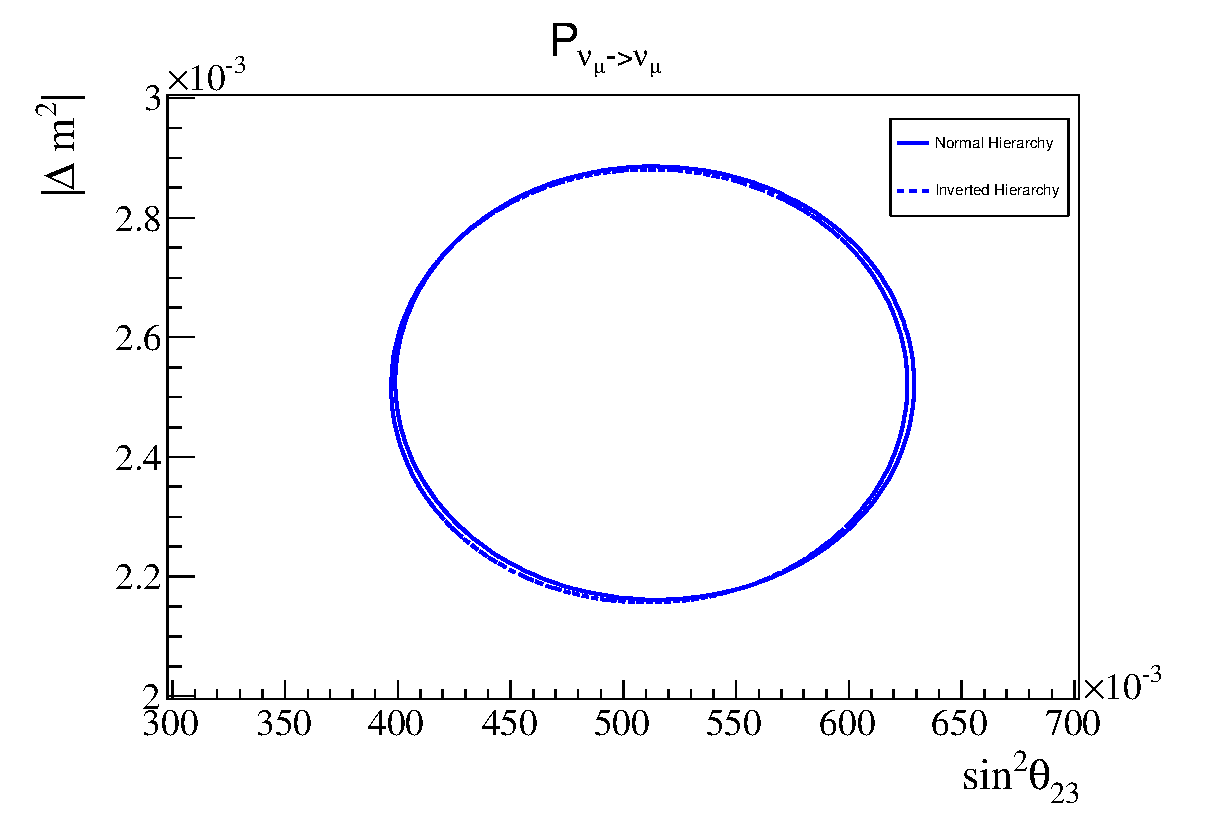
\includegraphics[width=0.5\textwidth]{images/appendix/fogliandlisi/OscProbNHIHFL.eps}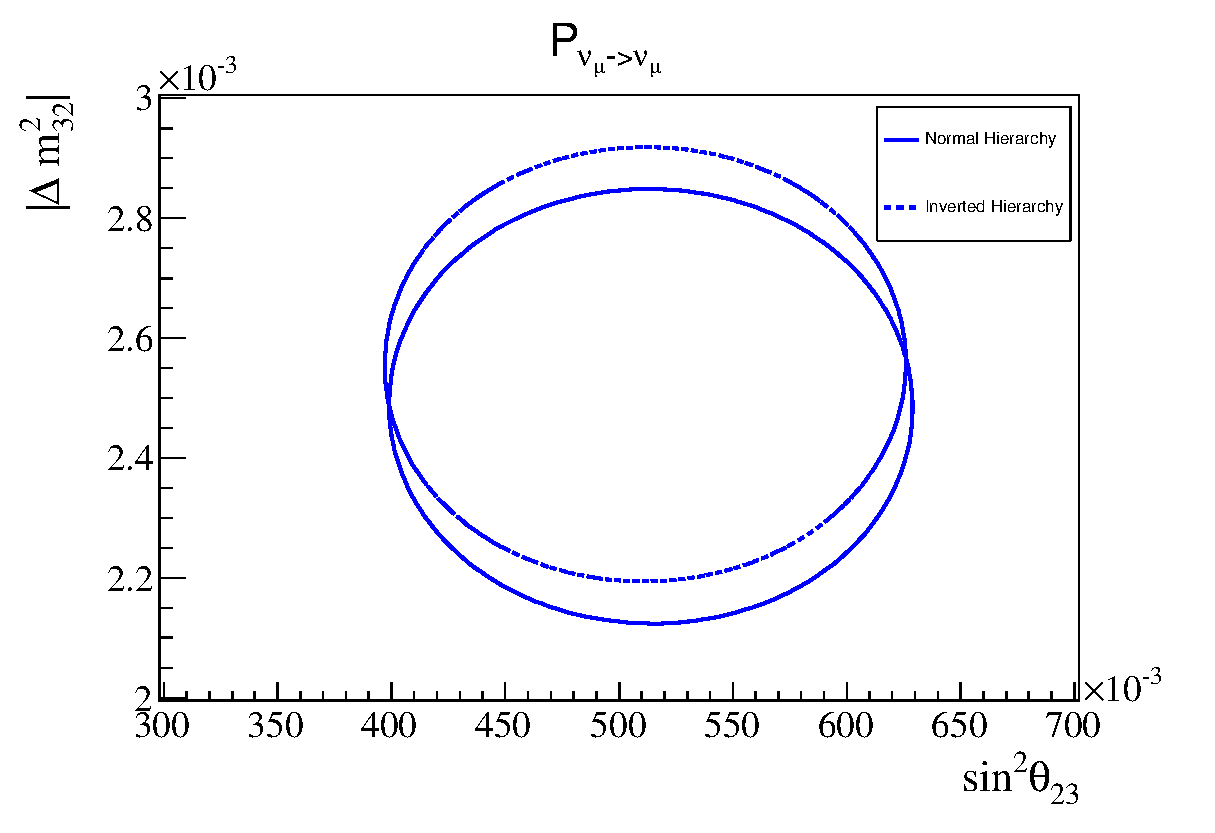
\includegraphics[width=0.5\textwidth]{images/appendix/fogliandlisi/OscProbNHIHNoFL.eps}
\caption{
P($\nu_{\mu}\rightarrow\nu_{\mu}$) survival probability in the
2-dimensional oscillation parameter spaces ($\sin^{2}\theta_{23}$, $|\Delta m^{2}|$) (left) and ($\sin^{2}\theta_{23}$, $|\Delta m_{32}^{2}|$) (right)
for a fixed value of P($\nu_{\mu}\rightarrow\nu_{\mu}$) = 0.05.
}
\label{fig:numusurvfl}
\end{center}
\end{figure}

Figure \ref{fig:truechisqfl} shows the true $\chi^{2}$ surface for the single ring $\mu$-like sample of the Run1+2+3 dataset in the
2-dimensional oscillation parameter spaces ($\sin^{2}\theta_{23}$, $|\Delta m^{2}|$) (left) and ($\sin^{2}\theta_{23}$, $|\Delta m_{32}^{2}|$) (right).
A contour is drawn in this figure for a fixed value of true $\chi^{2}=60$ in order to compare a line of points with the same vale of true $\chi^{2}$
in both mass hierarchies. The behaviour in the plots in Figure \ref{fig:truechisqfl} is exactly the same as observed in Figure \ref{fig:numusurvfl}.


\begin{figure}[htbp]
\begin{center}
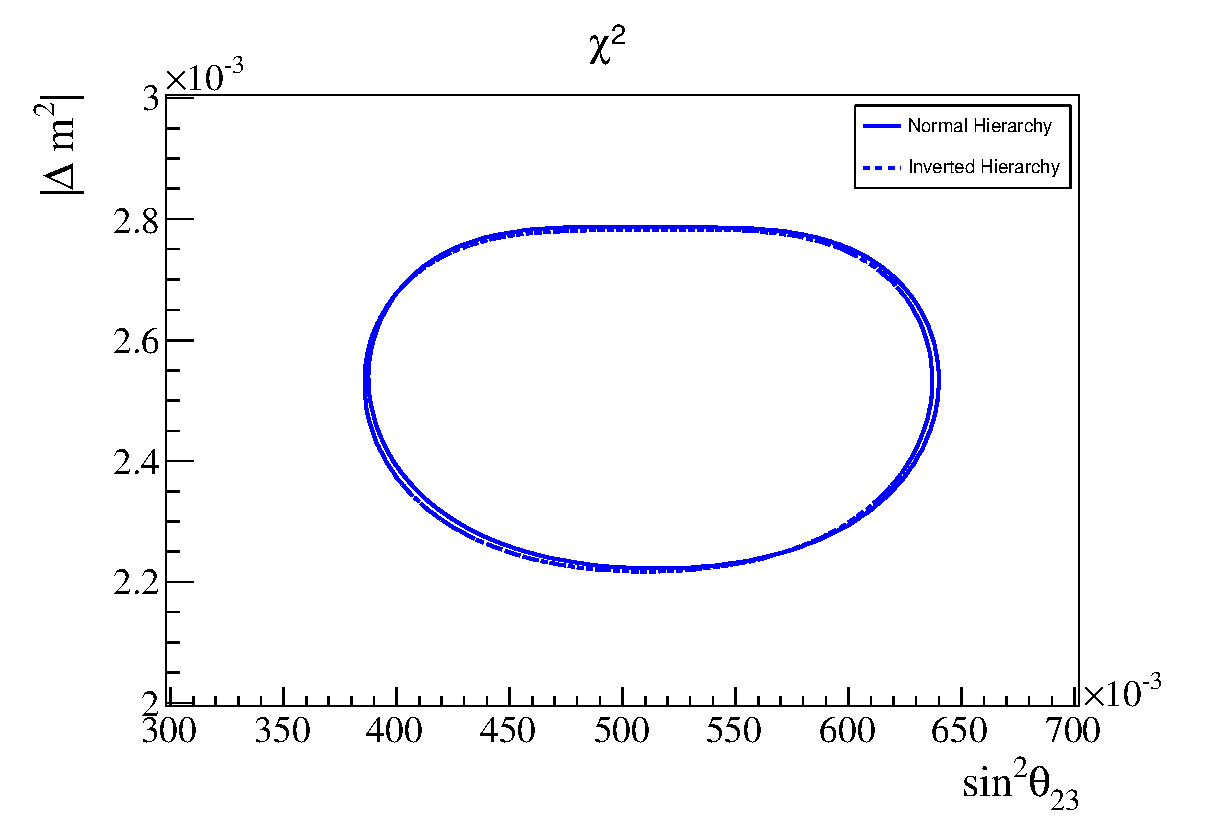
\includegraphics[width=0.5\textwidth]{images/appendix/fogliandlisi/TrueChisqNHIHFL.eps}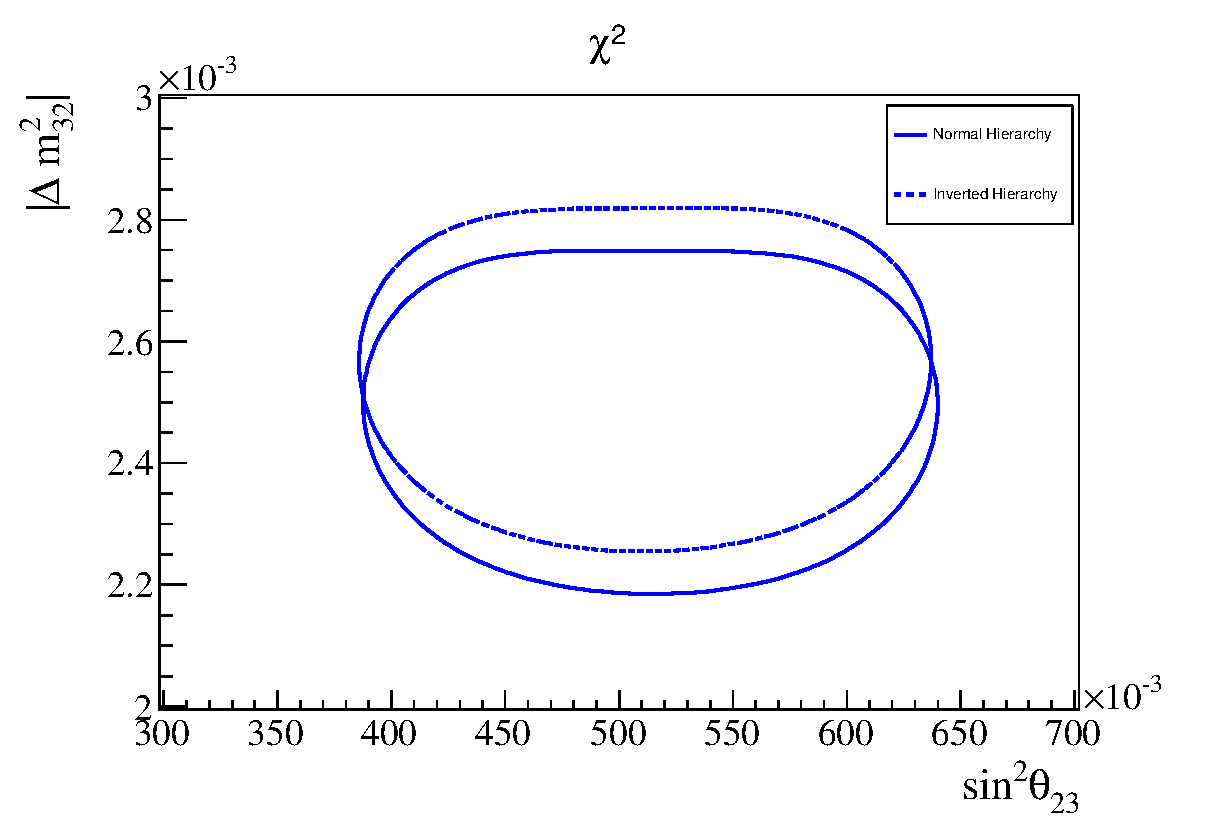
\includegraphics[width=0.5\textwidth]{images/appendix/fogliandlisi/TrueChisqNHIHNoFL.eps}
\caption{
True $\chi^{2}$ surface for the single ring $\mu$-like sample of the Run1+2+3 dataset in the 2-dimensional oscillation parameter spaces ($\sin^{2}\theta_{23}$, $|\Delta m^{2}|$) (left) 
and ($\sin^{2}\theta_{23}$, $|\Delta m_{32}^{2}|$) (right) for a fixed value of true $\chi^{2}=60$.
}
\label{fig:truechisqfl}
\end{center}
\end{figure}

Figure \ref{fig:disapcontourfl} shows the 90\% CL for the Run1+2+3 dataset in the
2-dimensional oscillation parameter spaces ($\sin^{2}\theta_{23}$, $|\Delta m^{2}|$) (left) and ($\sin^{2}\theta_{23}$, $|\Delta m_{32}^{2}|$) (right)
for the stand-alone $\nu_{\mu}$ disappearance analysis with Normal Hierarchy (solid line) and Inverted Hierarchy (dashed line) with the constant $\Delta \chi^{2}$ method.
As shown in this figure, an artificial difference between the contours in both hierarchies appears when using ($\sin^{2}\theta_{23}$, $|\Delta m_{32}^{2}|$)
because the quantity $|\Delta m_{32}^{2}|$ has a different meaning in each mass hierarchy (it is the largest mass-squared splitting in IH whereas the second largest in NH). 
There is almost no difference between the contours in both hierarchies when using the Fogli and Lisi convention  ($\sin^{2}\theta_{23}$, $|\Delta m^{2}|$) .

\begin{figure}[htbp]
\begin{center}
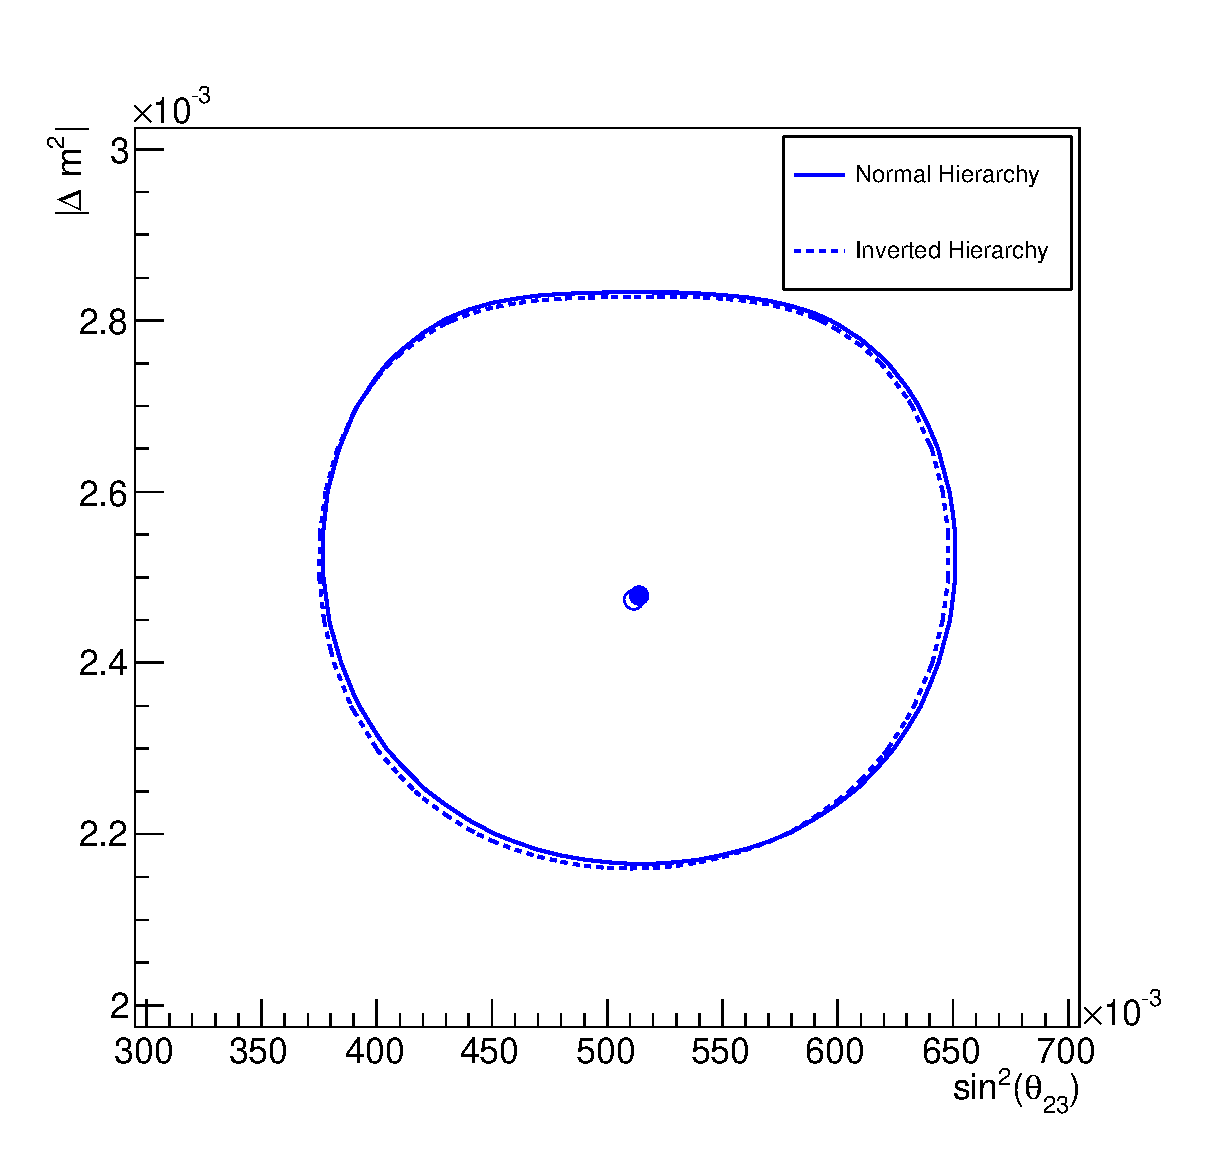
\includegraphics[width=0.5\textwidth]{images/appendix/fogliandlisi/ContourNHIHFL.eps}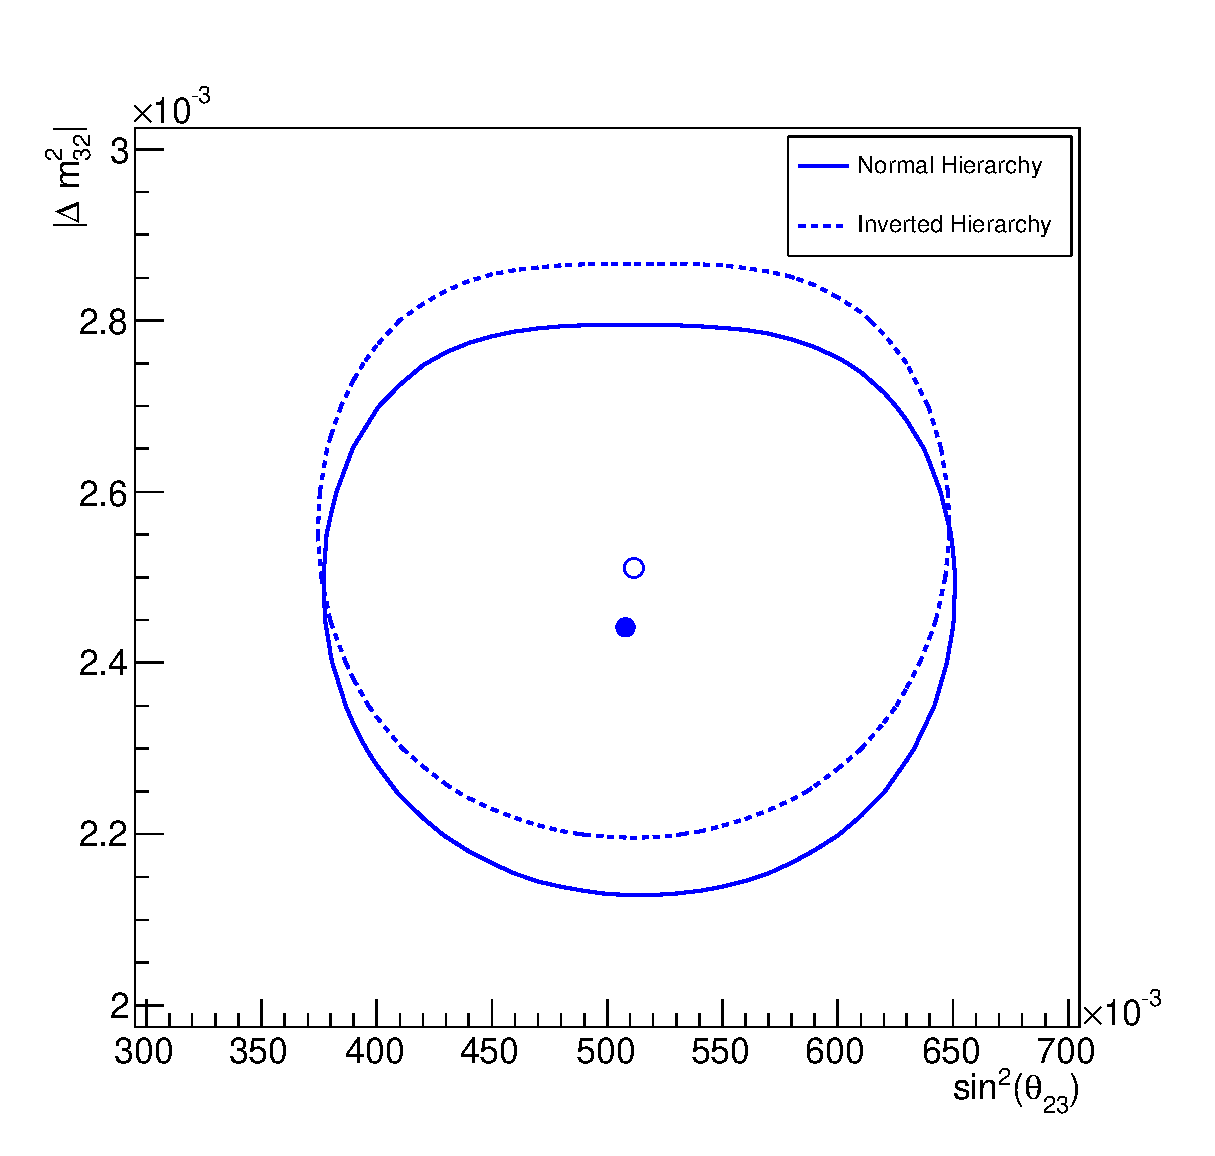
\includegraphics[width=0.5\textwidth]{images/appendix/fogliandlisi/ContourNHIHNoFL.eps}
\caption{
90\% CL for the Run1+2+3 dataset in the 2-dimensional oscillation parameter spaces ($\sin^{2}\theta_{23}$, $|\Delta m^{2}|$) (left) and ($\sin^{2}\theta_{23}$, $|\Delta m_{32}^{2}|$) (right)
for the stand-alone $\nu_{\mu}$ disappearance analysis with Normal Hierarchy (solid line) and Inverted Hierarchy (dashed line) with the constant $\Delta \chi^{2}$ method.
}
\label{fig:disapcontourfl}
\end{center}
\end{figure}
